% !TEX root =  master.tex
\chapter{Prototypische Umsetzung des Kubernetes Clusters}
\label{Umsetzung_K8s_Cluster}
In den folgenden Unterkapiteln erfolgt die Erläuterung der praktischen Umsetzung des in Kapitel \ref{Konzeption_K8s_Cluster} vorgestellten Konzeptes zur prototypischen Portierung der \ac{SaaS}-Lösung in ein Kubernetes Cluster. Des Weiteren wird die Provisionierung des Kubernetes Clusters und die hierfür benötigten Infrastruktur aufgezeigt. Zudem werden die für die praktische Umsetzung benötigten nativen Kubernetes-Objekte sowie die hierfür verwendeten Tools erläutert.
\section{Provisionierung des Kubernetes Clusters}
\label{Umsetzung_Provisionierung_Cluster}
Für die praktische Umsetzung der prototypischen Portierung wurde ein mittels des Gardener Projektes provisioniertes Kubernetes Cluster verwendet. Die einmalige Provisionierung und Konfiguration des Clusters wurden im Gardener Dashboard durchgeführt. Dabei wurden Konfigurationen, wie beispielsweise die Verknüpfung mit dem \ac{IaaS}-Konto und die verwendete Infrastruktur vorgenommen.\\
Als Infrastruktur dienten am Anfang der praktischen Umsetzung zwei \acsp{VM} der \ac{GCP} vom Typ \textbf{n1-standard-4}. Jedoch wurden diese aufgrund von mangelnden Rechenressourcen im Laufe der Umsetzung auf vier Instanzen mit jeweils 50 \ac{GB} persistentem Speicherplatz verdoppelt. \\
Die Infrastruktur der \ac{GCP} wird in der Zone \textbf{europe-west1-d} bereitgestellt. Diese befindet sich in Belgien und wurde wegen der günstigeren Gesamtkosten im Vergleich zu einem Rechenzentrum in Frankfurt ausgewählt.
\\
Als Betriebssystem der \acsp{VM} kommt hierbei CoreOs zum Einsatz, da dies Teil der Open Source Community ist und sich hinsichtlich des geringen Speicherplatzbedarfs optimal für die Bereitstellung skalierbarer Containeranwendungen eignet. \\ 
Das Cluster basiert auf der Kubernetes Version 1.16.4, welche zum Startzeitpunkt der vorliegenden Thesis die aktuellste Version gewesen ist.\\
Außerdem generiert Gardener automatisch einen Domainnamen, welcher für den externen Zugriff auf Ingress Services des Clusters verwendet werden kann. Die von Gardener bereitgestellte \ac{URL} lautet wie folgt: \url{*.ingress.k8s-sb.subbilling.shoot.canary.k8s-hana.ondemand.com}.\\
\newpage
Zusätzlich wurde der Open Source Service Mesh Istio auf dem Kubernetes Cluster installiert.\footnote{Guide zur Installation von Istio: \url{https://istio.io/docs/setup/install/istioctl/}} Dabei wurde erstmalig das standardmäßige Konfigurationsprofil \textbf{Demo} verwendet, da es die größte Auswahl an zusätzlichen Tools speziell für das Monitoring beinhaltet.\footnote{Übersicht der Konfigurationsprofile von Istio: \url{https://istio.io/docs/setup/additional-setup/config-profiles/}}\\ 
Generell sind Service Meshes Plattformen, die zur Lösung von typischen Herausforderungen einer Microservice-Architektur entstanden sind. Zu den Herausforderungen gehören beispielsweise Load Balancing, Service Discovery, und End-To-End Authentifizierung. Das Lösen der zuvor genannten Herausforderungen wurde innerhalb des Prototyps weitestgehend umgesetzt und wird in den folgenden Kapiteln erläutert.\\   
Der Service Mesh Istio setzt nativ auf der Kubernetes Plattform auf und bietet mit der eigenen \ac{API} zusätzliche Objekte zum Lösen der zuvor genannten Herausforderungen an.\autocite[Vgl.][]{IstioAuthors.2019b}
\\
Aus technischer Sicht wird Istio mittels des \textbf{Sidecar Patterns} in die Kubernetes Plattform integriert. Dabei wird automatisch in jedem Kubernetes Pod ein weiterer Container hinzugefügt. Dieser Container dient als \textbf{Envoy-Proxy}, der alle eingehenden und ausgehenden Anfragen abfängt und die vollständige Kommunikation zwischen den Microservices übernimmt.\footnote{Weitere Informationen zu Envoy: \url{https://www.envoyproxy.io/docs/envoy/latest/intro/what_is_envoy}} Zudem bietet der Proxy-Container weitere Funktionalitäten, wie etwa Load Balancing, End-To-End Authentifizierung oder auch \textbf{Tracing}.\autocite[Vgl.][S. 82-83]{Sharma.2020} Die zuvor genannten Funktionalitäten werden jeweils in den folgenden Unterkapiteln erneut aufgegriffen und erläutert.
Eine beispielhafte Darstellung des Sidecar Patterns ist der Abbildung \ref{sidecar_pattern} zu entnehmen.
\begin{figure}[h]
	\begin{center}
		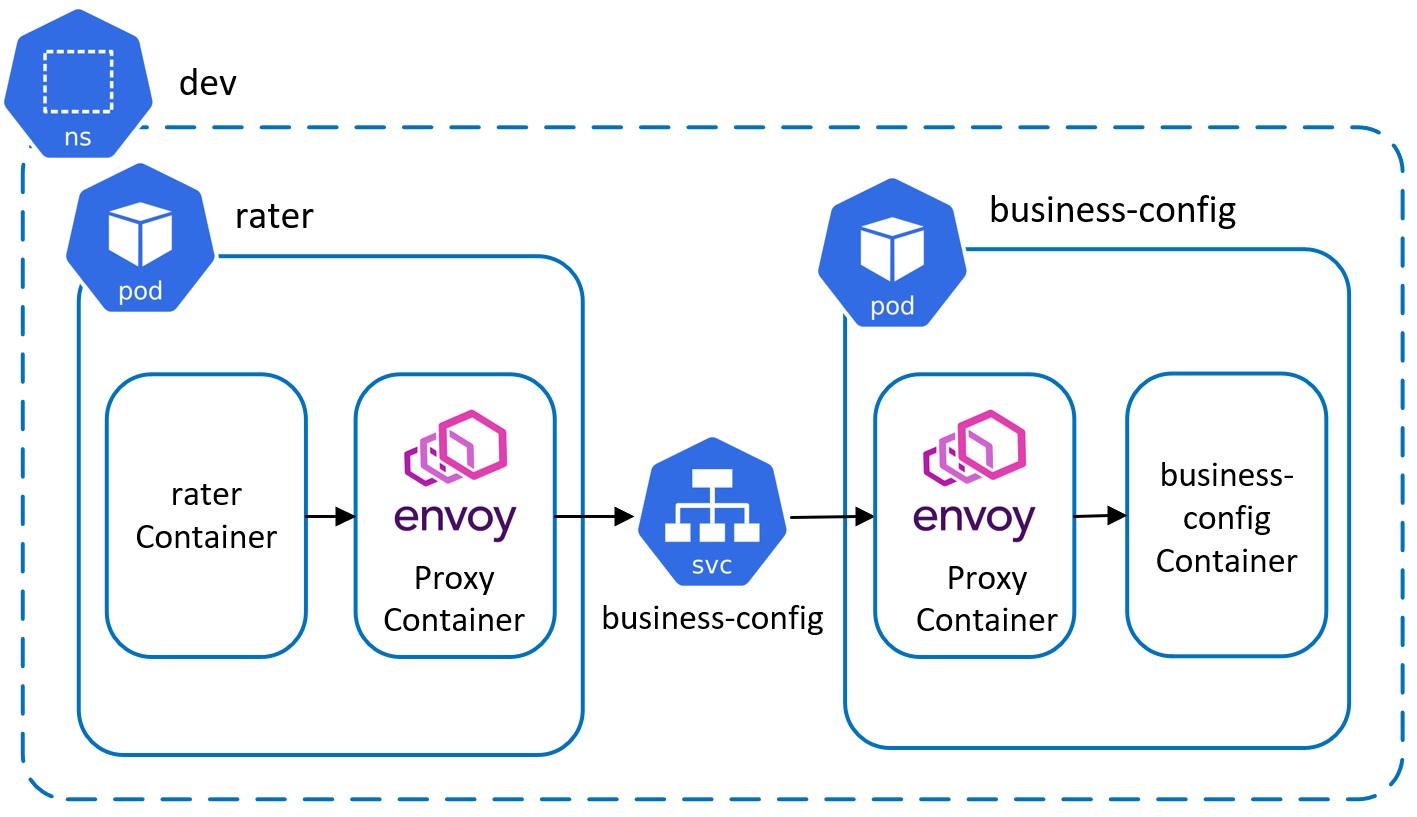
\includegraphics[width=13cm]{img/Sidecar_Pattern.JPG}
		\caption[Istio Sidecar Pattern]{Istio Sidecar Pattern (Eigene Abbildung)}
		\label{sidecar_pattern}
	\end{center}
\end{figure}
\newpage
\section{Bereitstellung ausgewählter Microservices}
\label{Umsetzung_Bereitstellung_Microservices}
Wie bereits in Kapitel \ref{Konzeption_Auswahl_Microservices} konzeptioniert, dienen der Rater- und der Business-Config-Microservice zur prototypischen Portierung von SAP Subscription Billing auf ein Kubernetes Cluster. Für die Portierung des Rater-Microservices wurden zusätzlich eine lokale PostgreSQL-Datenbank sowie der RabbitMQ Message Broker benötigt. Der Business-Config-Microservice hingegen benötigt eine MongoDB-Datenbank und verwendet ebenso RabbitMQ. \\
Die Bereitstellung der zuvor aufgezählten Komponenten wurde erstmalig mit einem Kubernetes \textbf{Deployment} durchgeführt.\\
Ein Kubernetes Deployment basiert generell auf dem \textbf{Replica Set}. Dieses ist ein Controller, der Pods aus einem Pod Template generiert und die Anzahl an bereitgestellten Replikaten eines Pods überwacht. Dabei werden bei Abweichungen Pods terminiert oder zusätzlich gestartet. Grundsätzlich baut ein Deployment auf den Funktionalitäten eines Replica Sets auf und erweitert diese besonders um weitere Funktionalitäten für die Aktualisierung der Anwendung. Dabei kann zum Beispiel ein \textbf{Rollback} der aktualisierten Anwendung durchgeführt werden, welches die Version der Anwendung auf die zuletzt funktionsfähige Version zurückführt und die Pods aktualisiert.\autocite[Vgl.][S. 118, 276]{Luksa.2018}
\\
Für die Bereitstellung der eigentlichen Microservices wurden \textbf{Stateful Sets} verwendet.\\
Ein Stateful Set basiert, wie auch das Deployment, grundsätzlich auf dem Replica Set. In Abgrenzung zu einem Deployment sind die mittels eines Stateful Sets bereitgestellten Pods jedoch statusbehaftet. Dies bedeutet, dass ein Pod eine feste Identität hat, die auch bei einem Neustart wiederhergestellt wird.\autocite[Vgl.][S. 311-312]{Luksa.2018} Die Entscheidung für die Verwendung von Stateful Sets wurde aufgrund der einfacheren Möglichkeiten zum lokalen Testen, Überwachen und Debuggen gewählt, da der Domainname der einzelnen Pods auch bei einer erneuten Bereitstellung eindeutig bleibt.\\
Aus diesen Gründen wurden während der praktischen Umsetzung alle Bereitstellungen, welche zuvor mit einem Deployment umgesetzt wurden, auf Stateful Sets umgestellt, darunter auch die Bereitstellung der Datenbanken und des RabbitMQ Message Brokers.\\
\\
Die clusterinterne Zurverfügungstellung der Pods wurde unter Zuhilfenahme eigenständiger \textbf{Services} realisiert. Ein Service dient als interne Netzwerkschnittstelle für ein logisches Set an Pods. Dadurch können die Service Discovery Funktionalitäten abgedeckt werden, da alle Anfragen an den gleichbleibenden Domainnamen des Service geschickt werden können. Hierfür wurde jeweils pro Pod ein Service erstellt. Eine beispielhafte Implementierung des für den Rater-Microservice erstellten Service ist aus dem Quelltext \ref{quellcode_rater_service} zu entnehmen. \\
Dabei wird bei der Servicedefinition festgelegt, unter welchem Port der Service zur Verfügung steht und an welches Set von Pods die Anfragen weitergeleitet werden sollen. Hierbei erfolgt die Auswahl der Pods über den Labelselektor, der mit den Labels der Pods übereinstimmen muss. Diese Abstraktion hat den Vorteil, dass selbst bei Änderungen am Namen des Pods oder dessen Aktualisierung auf eine neue Version keine Änderungen am Service durchgeführt werden müssen.\\
Jedoch ist zu beachten, dass durch die Verwendung von Stateful Sets ein besonderer Servicetyp für die beiden Microservices benötigt wird. Da diese Pods eine unveränderliche Netzwerkidentität haben, sollten sogenannte \textbf{Headless Services} verwendet werden. Diese entsprechen grundsätzlich den normalen Services und unterscheiden sich lediglich seitens des Nichtvorhandenseins einer clusterinternen \ac{IP}-Adresse. Damit wird im clusterinternen \ac{DNS}-Dienst die direkte \ac{IP}-Adresse der Pods hinterlegt. Demzufolge wird die direkte Kommunikation mit dem Pod selbst ohne Umwege über einen Service ermöglicht. Des Weiteren ist die generelle Verwendung von normalen Services ebenso möglich. Jedoch kann dabei nicht sichergestellt werden, dass bei einer Anwendung, welche mit mehreren Replikaten bereitgestellt ist, immer mit dem gleichen Pod kommuniziert wird.\\
Zusätzlich sollte bei der Verwendung von Headless Services berücksichtigt werden, dass dadurch die Load Balancing Funktionalität der Services umgangen wird.\autocite[Vgl.][]{KubernetesAuthors.20200115}\\
\\
Innerhalb der praktischen Umsetzung wurden keine Headless Services verwendet, da die für den Prototyp verwendeten Komponenten jeweils nur mit einem Replikat bereitgestellt wurden, um den Bedarf an Rechenressourcen zu minimieren.\\
Zudem wurden für die beiden Microserives \textbf{Horizontal Pod Autoscaler} Controller erstellt, welche abhängig von der aktuellen \ac{CPU}-Auslastung der bereitgestellten Podreplikate automatisch zusätzliche Replikate bereitstellen. Hierbei wurde zum Beispiel für den Rater-Microservice festgelegt, dass wenn die \ac{CPU}-Auslastung höher als 85 \% ist, ein weiteres Podreplikat bereitgestellt werden soll.\\
\\
Für die Sicherstellung der Datenpersistenz wurden für die PostgreSQL- und die MongoDB-Instanzen jeweils \textbf{Persistent Volume Claims} definiert. Diese veranlassen die Bereitstellung von \textbf{Persistent Volumes}, welche auf nicht flüchtigem Standardspeicher der \ac{GCP} basieren. Die Typdefinition des Speichermediums wurde mit Hilfe von einer \textbf{Storage Class} umgesetzt. Diese wird direkt mit dem Persistent Volume Claim verknüpft, sodass dieser auf das in der Storage Class definierte Speichermedium zurückgreift. Darüber hinaus wird im Persistent Volume Claim die benötigte Speichergröße des Persistent Volumes definiert. \autocite[Vgl.][S. 196, 198-199]{Luksa.2018}\\
\\
In den Deployment- und Stateful Set-Objekten wurde jeweils die \acsp{URL} der in der Image Registry bereitgestellten Docker-Images angegeben. Zusätzlich wurde ein \textbf{Secret} angelegt, welches die Anmeldeinformationen für die Docker Registry verschlüsselt abspeichert. Dieses Secret wird für die Bereitstellung der Pods verwendet, da für die Verwendung der Docker-Images die Autorisierung gegenüber der SAP eigenen Image Registry benötigt wird.\\
Bei der Bereitstellung der im Deployment definierten Container wird das Docker-Image von der lokalen Container Engine Docker heruntergeladen und anschließend in einem Pod auf dem Kubernetes Cluster bereitgestellt.\\
Die für die beiden Microservices benötigten Docker-Images wurden erstmalig manuell auf dem lokalen Rechner gebaut und in die Image Registry hochgeladen. Jedoch wurde dieser Schritt mit Hilfe der Integration in die \ac{CI}/\ac{CD}-Pipeline vollständig automatisiert. Die Erläuterung der Integration erfolgt in Kapitel \ref{Umsetzung_CI_CD_Integration}. \\
Für die Bereitstellung der RabbitMQ-\footnote{Offizielles RabbitMQ Docker-Image: \url{https://hub.docker.com/_/rabbitmq}}, MongoDB-\footnote{Offizielles MongoDB Docker-Image: \url{https://hub.docker.com/_/mongo}} und PostgreSQL-Pods\footnote{Offizielles PostgreSQL Docker-Image: \url{https://hub.docker.com/_/postgres}} wurde jeweils die aktuellste Version des offiziellen Docker-Images verwendet.\\
Beispielhafte Manifestdateien aller zuvor erwähnten Kubernetes \ac{API}-Objekte und ein beispielhaftes Dockerfile sind im Anhang in Kapitel \ref{quellcode_bereitstellung_microservices} zu finden.


\section{Verschiedene Landschaften}
\label{Umsetzung_Landschaften}
Die erstmalige Umsetzung des Routings der externen Anfragen wurde mittels des Ingress Services von Kubernetes umgesetzt. Eine beispielhafte Manifestdatei für einen Ingress Service ist aus dem Quelltext \ref{quellcode_ingress_service} im Anhang zu finden. Dabei wird innerhalb des Service der extern verfügbare Hostname, wie etwa \url{rater.ingress.k8s-sb.subbilling.shoot.canary.k8s-hana.ondemand.com} und eine Routingregel für die Weiterleitung der an den Hostnamen gesendeten Anfragen definiert. Mit der Routingregel wurde zum Beispiel die Weiterleitung an den erstellten Kubernetes Service des Rater-Microservices festgelegt.\\
\\
Wie in Kapitel \ref{Konzeption_Landschaften} erläutert, wurde das Konzept für das Routing der externen Anfragen durch die Verwendung der folgenden von Istio angebotenen Objekte erweitert:
Virtual Services, Gateways und Destination Rules. 
\\
Ein Istio Virtual Service entspricht grundsätzlich den Services von Kubernetes. Jedoch können mit einem Virtual Service durchaus komplexere Routingregeln definiert werden. 
\newpage
Für die praktische Umsetzung des Anfragenroutings wurden Virtual Services benutzt, da diese unter anderem für das mandantenabhängige Routing der Anfragen, basierend auf den \ac{HTTP}-Headern der Anfrage, verwendet werden können. 
Ein weiterer Vorteil von Virtual Services ist im Vergleich zu den nativen Kubernetes Services zum Beispiel die Möglichkeit eines gewichteten Routings auf unterschiedliche Versionen der bereitgestellten Anwendung.\autocite[Vgl.][S. 153]{Sharma.2020} Damit kann beispielsweise \textbf{Canary Releasing} umgesetzt werden. Dies ist eine Aktualisierungsstrategie, bei der die aktualisierte Anwendung erstmalig an beispielshalber fünf Prozent der Anwender getestet wird, bevor sie für alle Anwender zur Verfügung steht.\autocite[Vgl.][]{Sato.2014}\\ 
\\
Eine Destination Rule wird für das versionsabhängige Routing der Anfragen benötigt. Dabei werden innerhalb der Destination Rule die Subsets der Services definiert, welche sich in ihren Versionen unterscheiden. So ist es durch die Verwendung von Versionslabels möglich, mit ausschließlich einem Service das Routing zu mehreren Versionen einer bereitgestellten Anwendung durchzuführen.
Voraussetzung für das versionsabhängige Routing ist das Vorhandensein der Versionsangabe der Anwendung mittels eines einfachen Kubernetes Labels.\\
Ein Istio Gateway ist vergleichbar mit einem Kubernetes Ingress Service. Dieser dient als Load Balancer mit einer externen Schnittstelle, der die Anfragen an einen Virtual Service weiterleitet. Jedoch unterstützt ein Gateway, im Gegensatz zu einem Ingress Service, keine Routingregeln. Er definiert ausschließlich einen Service, der externe Anfragen an die hinterlegte Hostadresse und die festgelegten Ports zulässt und weiterleitet.\autocite[Vgl.][]{IstioAuthors.2019}\\
Eine Gesamtübersicht, der für das mandantenabhänge Routing der Anfragen implementierten Objekte ist der Abbildung \ref{picture_request_routing} zu entnehmen.
\\
Bei dem dargestellten und praktisch umgesetzten Konzept für das Anfragenrouting wird abhängig vom Mandanten das Routing der Anfrage an den Service in den dafür vorgesehen Kubernetes Namespace durchgeführt. Der Mandant sieht exemplarisch wie folgt aus: \textbf{revcloud-dev-eu10-<teamname>}. Hierfür wurden Routingregeln mittels der Istio Virtual Services definiert, welche abhängig von \ac{HTTP}-Headern die Weiterleitung der Anfrage an den eigentlichen Kubernetes Service durchführen.\\
\\
Wie bereits in Kapitel \ref{Konzeption_Landschaften} erläutert, wurde die Isolation der Landschaften sowie die unerwünschte Kommunikation der Pods aus dem gleichen Namespace mit Network Policies konzeptioniert.
Bei der praktischen Umsetzung wurde jeweils eine Network Policy per Pod in einen Namespace implementiert. Eine beispielhafte Manifestdatei der Network-Policy für den Business-Config-Microservice ist aus dem Quelltext \ref{quellcode_verschiedene_landschaften} zu entnehmen.
\begin{figure}[h]
	\begin{center}
		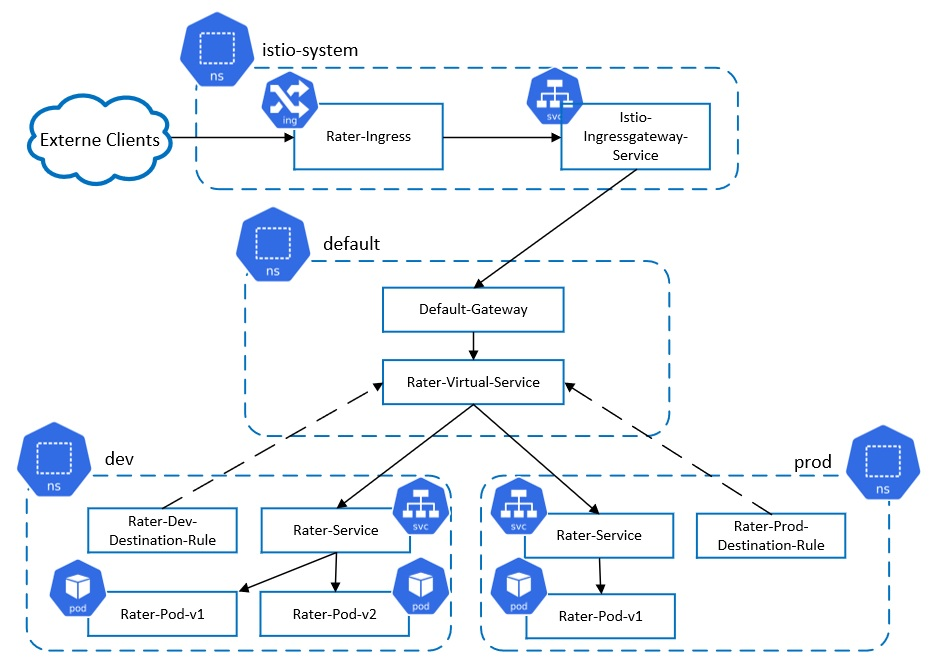
\includegraphics[width=16cm]{img/Landscape_Routing.JPG}
		\caption[Zentrales Routing der Anfragen mit mehreren Landschaften]{Zentrales Routing der Anfragen mit mehreren Landschaften \\(\cite[Eigene Abbildung in Anlehnung an][S. 170]{Sharma.2020})}
		\label{picture_request_routing}
	\end{center}
\end{figure}
\\
Innerhalb der Network Policies wurde die Kommunikation sowohl auf Namespace-Ebene als auch auf Pod-Ebene eingeschränkt. Dabei werden zum Beispiel für den Business-Config-Microservice ausschließlich Anfragen, welche aus dem gleichen Namespace und von Pods, die mit den hinterlegten Labels übereinstimmen, zugelassen.\\
Dadurch konnte die vollständige Unterbindung nicht vorgesehener Kommunikation zwischen den Microservices als auch den Datenbanken umgesetzt werden.
\\
Insgesamt konnte mit Hilfe der Routingobjekte von Istio die Funktionalität für das Routing des aktuell eingesetzten Landscape-Routers vollständig abgedeckt und somit ersetzt werden. Zudem sind weitere Funktionalitäten, wie beispielsweise das zuvor erläuterte Canary Releasing Konzept, möglich.\\
Die beispielhafte Implementierung der zuvor genannten Istio-Objekte für das Anfragenrouting an den Rater-Microservice ist im Anhang unter dem Kapitel \ref{quellcode_verschiedene_landschaften} zu finden.

\section{Integration in die \acs{CI}/\acs{CD}-Pipeline}
\label{Umsetzung_CI_CD_Integration}
Wie in Kapitel \ref{Konzeption_integration_ci_cd_pipeline} konzeptioniert, wurde die Automatisierung der Anwendungsaktualisierung mittels der Integration in die Jenkins \ac{CI}/\ac{CD}-Pipelines umgesetzt.\\
Grundsätzlich existierte zum aktuellen Zeitpunkt der Thesis in dem Subscription Billing Projekt pro Microservice eine eigene Pipeline. Diese wird bei jeder Änderung am hinterlegten Git Repository automatisch ausgeführt. Dabei ist eine Pipeline ein umfangreicher Prozess, welcher die einzelnen \ac{CI}/\ac{CD}-Schritte abarbeitet. Die Deklaration der Pipeline und deren Schritte erfolgt anhand eines \textbf{Jenkinsfiles}.
Eine Pipeline kann, wie in Abbildung \ref{picture_jenkins_pipeline} zu sehen ist, in Stages unterteilt werden, welche zur Gruppierung einzelner Schritte genutzt werden können.\autocite[Vgl.][]{JenkinsAuthors.20190308}\\
Für die Integration der Bereitstellung der Microservices auf das Kubernetes Cluster wurden die Jenkins-Pipelines jeweils um die Stage \textbf{K8s Deployment} erweitert.\\
Die hierfür benötigte Erweiterung des Jenkinsfiles ist im Anhang in Kapitel \ref{quellcode_rater_jenkinsfile} zu finden. Ein Überblick der einzelnen Stages der Pipeline des Rater-Microservice ist der Abbildung \ref{picture_jenkins_pipeline} zu entnehmen. 
\\
\begin{figure}[h]
	\begin{center}
		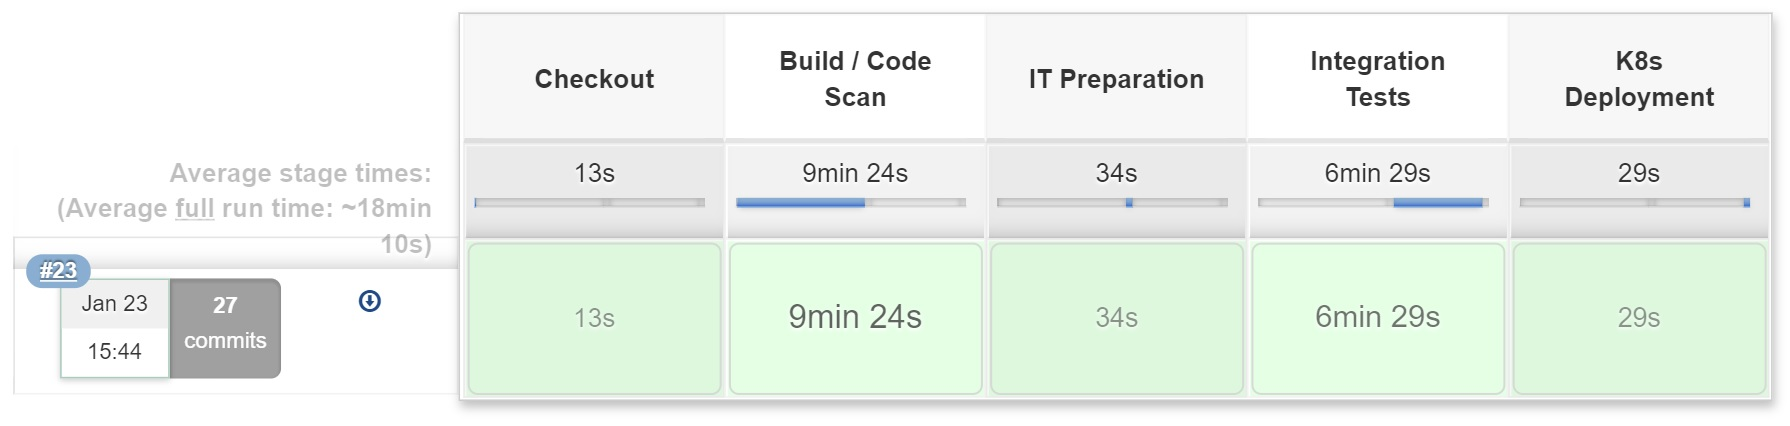
\includegraphics[width=16cm]{img/Jenkins_Pipeline.JPG}
		\caption[Übersicht Stages der Jenkins-Pipeline]{Übersicht Stages der Jenkins-Pipeline\\(Abbildung stammt aus der der Jenkins Pipeline)}
		\label{picture_jenkins_pipeline}
	\end{center}
\end{figure}
\\
Innerhalb der K8s-Deployment-Stage wurden die folgenden Schritte konzeptioniert und implementiert. 
\begin{enumerate}
	\item Bauen des Docker-Images mittels des Artefakts des Microservices, des Dockerfiles und der lokalen Container Engine Docker.
	\item Kennzeichnen des Docker-Images mit dem aktuellen Zeitstempel.
	\item Hochladen des Docker-Images auf die extern verfügbare Image Registry von SAP.
	\item Bereitstellen/Aktualisieren der im Skaffold-Manifest definierten Kubernetes \ac{API}-Objekte auf das Kubernetes Cluster.
\end{enumerate}
Die zuvor genannten Schritte der Stage wurden mit dem Skaffold Tool weiter automatisiert. 
Hierbei ist zu erwähnen, dass der Jenkins-Server selbst auf einem zusätzlichen Kubernetes Cluster bereitgestellt ist.\\ 
In der Pipeline werden jeweils Pods zur Bearbeitung der definierten Stages und deren Jobs generiert. Für die \textbf{K8s Deployment} Stage wurde ein bereits vorhandenes Pod-Template um einen Skaffold Container erweitert. Neben dem Skaffold Tool besitzt der Pod beispielsweise auch einen Container mit der lokalen Container Engine Docker, welche zum Bauen und Hochladen des Docker-Images verwendet wird.\\
Des Weiteren ist zu beachten, dass ohne die Verwendung von Skaffold die Bereitstellung eines Kubernetes-Objektes aus einem Pod eines Clusters in ein anderes Kubernetes Cluster nicht ohne Workarounds möglich gewesen ist.\\
Jedoch konnten die benötigten Workarounds vollständig durch die Verwendung des Skaffold Tools ersetzt werden, da damit der für die Bereitstellung verwendete \textbf{kube-config} festgelegt werden kann. Dieser definiert in welchem Kubernetes Kontext und somit in welchem Kubernetes Cluster die Bereitstellung der definierten Objekte stattfinden soll.\autocite[Vgl.][]{SkaffoldAuthors.20200116}
Dadurch können mit Skaffold auch aus einem Kubernetes Cluster heraus Objekte in einem anderem Kubernetes Cluster bereitgestellt werden. Eine vereinfachte Darstellung des Bereitstellungsprozesses ist in Abbildung \ref{picture_ci_cd_process} zu sehen.\\
Ein weiterer Vorteil von Skaffold ist die Möglichkeit der sogenannten \textbf{skaffold dev}-Funktion. Diese Funktion ermöglicht die Aktualisierung der bereitgestellten Anwendung bei jeder Änderung des Quellcodes. Dies eignet sich besonders in Kombination mit der Verwendung eines Git Repositories. Hierbei kann Skaffold bei jeder Aktualisierung des Git Repositories die automatische Aktualisierung der Anwendung starten.\autocite[Vgl.][]{SkaffoldAuthors.20200116b}\\
Zum aktuellen Zeitpunkt ist die Verwendung dieses Features jedoch nicht geplant, da dies bereits mit der Jenkins-Pipelines umgesetzt wird.
\\
\begin{figure}[h]
	\begin{center}
		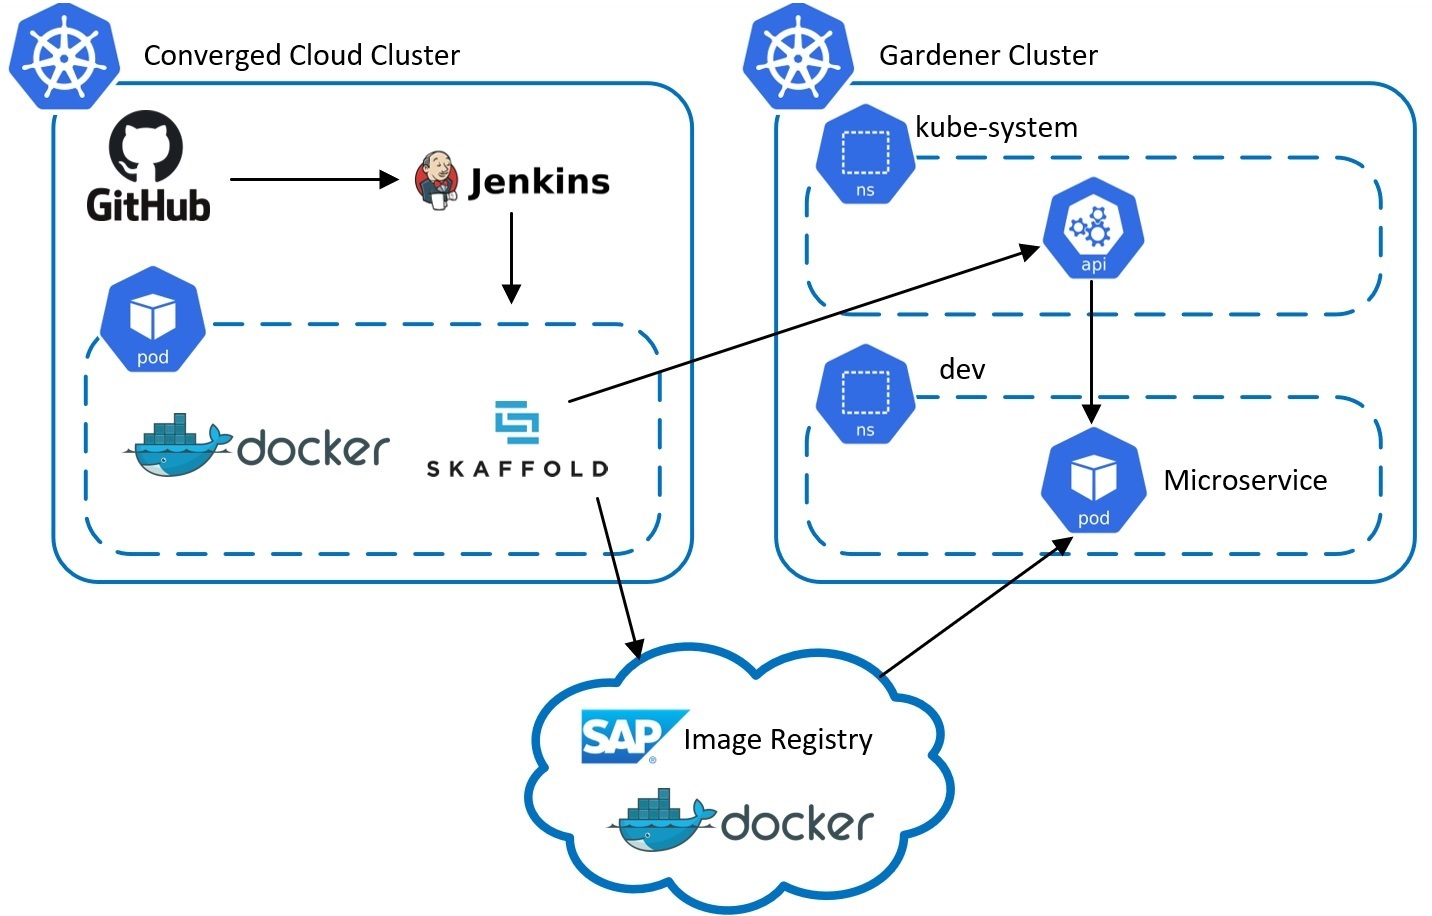
\includegraphics[width=16cm]{img/CI_CD_Integration.JPG}
		\caption[Übersicht Bereitstellungsprozess des Jenkins-Servers]{Übersicht Bereitstellungsprozess des Jenkins-Servers \\
			(Eigene Abbildung)}
		\label{picture_ci_cd_process}
	\end{center}
\end{figure}
\\
Generell ermöglicht Skaffold eine einheitliche Definition der beschriebenen Prozesse mittels einer einzigen Manifestdatei. \\
Eine beispielhafte Manifestdatei für den Rater-Microservice ist im Anhang in Kapitel \ref{quellcode_skaffold_rater} zu finden.\\
Ein zusätzlicher Vorteil von Skaffold ist die Möglichkeit der direkten Angabe des Namespaces bei der Verwendung des \textbf{skaffold run}-Kommandos. Dies kann mit dem \textbf{--namespace}-Tag durchgeführt werden. Dadurch soll bei dem gewählten Multi-Namespace-Konzept der für die Bereitstellung entsprechende Namespace per Tag angegeben werden. Auf diese Weise kann das Erstellen von duplizierten Manifestdateien, welche sich ausschließlich in der Definition des Namespaces unterscheiden, vermieden werden.\\
\newpage
Der Nachteil der Verwendung des Skaffold Tools ist ausschließlich die zusätzliche Manifestdatei für Skaffold und die benötigte Installation der lokalen Skaffold \ac{CLI}. Jedoch konnte dies mit Hilfe der Verwendung der automatischen Bereitstellung durch den Jenkins-Server auf einem zusätzlichen internen Kubernetes Cluster abgelöst werden.\footnote{Weitere Informationen zu Skaffold: \url{https://skaffold.dev/docs/}}\\ 

\section{Service-to-Service Kommunikation}
\label{Umsetzung_S2S_Kommunikation}
Wie bereits in Kapitel \ref{Konzeption_S2S_Kommunikation} erläutert, wurde die erste praktische Umsetzung der Kommunikation der Microservices untereinander mittels der nativen Kubernetes Services umgesetzt. Dabei wurde für jeden Microservice ein eigener Kubernetes Service erstellt, welcher als Schnittstelle für die eingehenden Anfragen anderer Microservices dient. Dabei erfolgt, wie in Kapitel \ref{Konzeption_S2S_Kommunikation} erläutert, die Weiterleitung der Anfragen mit Hilfe des im Service definierten Labelselektors. Eine beispielhafte Manifestdatei für den Service des Rater-Microservices ist aus dem Anhang im Quelltext \ref{quellcode_rater_service} zu finden.\\
\newpage
Da die Kubernetes Services jedoch nativ keine verschlüsselte Service-to-Service Kommunikation unterstützen, wurde das Konzept um die Virtual Services von Istio erweitert. Dabei wurden auch die zuvor implementierten Kubernetes Services benötigt und wiederverwendet.
\\
\begin{figure}[h]
	\begin{center}
		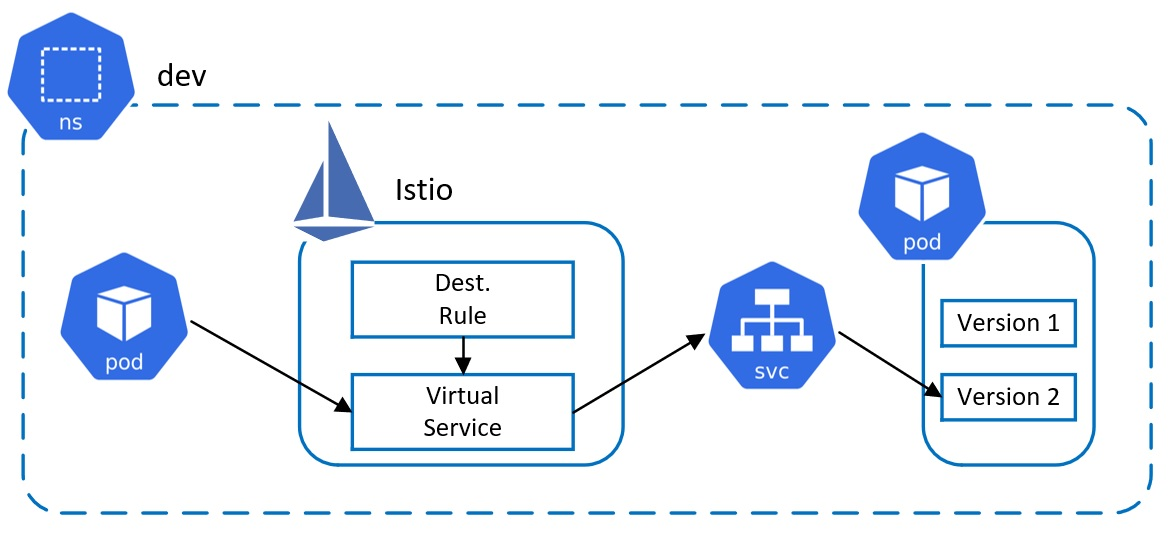
\includegraphics[width=16cm]{img/Istio_S2S_Kommunikation.JPG}
		\caption[Service-to-Service Kommunikation mit Istio]{Service-to-Service Kommunikation mit Istio\\
			(\cite[Eigene Abbildung in Anlehnung an][S. 145]{Sharma.2020})}
		\label{grafik_istio_s2s_kommunikation}
	\end{center}
\end{figure}
\\
Wie der vereinfachten Abbildung \ref{grafik_istio_s2s_kommunikation} zu entnehmen ist, fängt der Virtual Service als erste Komponente die Anfrage ab und leitet diese dann an den hinterlegten Kubernetes Service weiter. Dabei benötigt jeder Virtual Service eine Destination Rule, welche unter anderem die unterschiedlichen Versionen eines Service definiert. Zudem kann auch das für den Lastenausgleich eingesetzte Verfahren, wie beispielsweise das \textbf{Round Robin} Verfahren konfiguriert werden.\autocite[Vgl.][Destination Rule]{IstioAuthors.20191115} Weitere Informationen zu den möglichen Verfahren des Lastenausgleichs sind unter dem angegebenen Link zu finden.\footnote{Verfahren für den Lastenausgleich: \url{https://istio.io/docs/reference/config/networking/destination-rule/\#LoadBalancerSettings-SimpleLB}}\\
Innerhalb der Virtual Services können Routingregeln oder auch \textbf{Failover Szenarien} für auftretende Kommunikationsfehler hinterlegt werden.\\
Bei der praktischen Umsetzung des Prototyps wurde exemplarisch das Failover Szenario für den Virtual Service des Business-Config-Microservices implementiert. Dabei werden zum Beispiel bei einem Kommunikationsfehler mit dem \ac{HTTP}-Statuscode 503, 504 oder 505 jeweils drei erneute Kommunikationsversuche durchgeführt.\\
Eine beispielhafte Manifestdatei für einen Virtual Service ist aus dem Anhang im Quelltext \ref{quellcode_rater_vs} zu entnehmen.\\
\newpage
Generell ist jedoch zu berücksichtigen, dass die vom Service Mesh Istio verwendeten Virtual Services und Destionation Rules sich ausschließlich mittels den in Kapitel \ref{Umsetzung_Bereitstellung_Microservices} erläuterten Envoy Proxies in die interne Netzwerkkommunikation von Kubernetes einklinken können. Hierbei erfolgt die Angabe des Zielservices in einem Microservice weiterhin mit dem nativen Domainnamen des Kubernetes Services und es bedarf keiner Anpassungen an die vom Service Mesh Istio zusätzlich implementierten Objekte. Dies ist beispielsweise im Fall einer Anfrage, welche vom Rater-Microservice an den Business-Config-Microservice gesendet werden soll, die interne \ac{URL}: \url{http://business-config-svc:8080}.\\
\\
Der Hauptgrund für die Verwendung von Virtual Services ist jedoch die Unterstützung von \ac{mTLS}. Dies wurde einerseits mit Hilfe des Konfigurationsmanifests von Istio zentral für alle Services festgelegt. Dadurch wurde das clientseitige \ac{mTLS} aktiviert. Dabei legt die clientseitige Konfiguration von \ac{mTLS} fest, ob die Anfragen an die Services vom Endpunkt des Clients authentifiziert sein müssen.\\
Andererseits wurde die serverseitige Implementierung von \ac{mTLS} durch eine globale \textbf{Policy} umgesetzt. Diese definiert globale Vorschriften für die innerhalb des Clusters stattfindenden Netzwerkkommunikation und ist im Anhang aus dem Quelltext \ref{quellcode_globale_mtls_policy} zu entnehmen. \\
Mit Hilfe der serverseitigen Verwendung von \ac{mTLS} wird die eigentliche Verschlüsselung der Kommunikation umgesetzt.\autocite[Vgl.][Authentication policies]{IstioAuthors.20200106}\\
\\
Mit der Verschlüsselung der clusterinternen Kommunikation konnte bewiesen werden, dass der zentrale Credential Store Vault für die Absicherung der Kommunikation der Microservices nicht mehr benötigt wird. Dies kann dadurch begründet werden, dass bei \ac{mTLS} keine zusätzliche Authentifikation der Microservices mit Hilfe von Credentials eingesetzt werden muss.\\
Des Weiteren konnte die benötigte Service Discovery Funktionalität, die auf der \ac{CF} mit dem zusätzlichen Eureka-Service gelöst wurde, mittels der nativen Kubernetes Services und der Virtual Services von Istio ebenso abgedeckt werden. Dies hat den Vorteil, dass die generelle Verwaltung und der Betrieb des Eureka Services und des Credential Stores Vault bei der Verwendung von Kubernetes nicht mehr benötigt wird.\\
Zudem wurden mit Hilfe der Virtual Services die zuvor beschriebenen Failover Szenarien umgesetzt. Diese sichern beispielsweise eine durch Netzwerkprobleme bedingte, fehlgeschlagene Kommunikation ab.

\section{Monitoring und Logging}
\label{Umsetzung_Monitoring_Logging}
Zur Umsetzung des Loggingkonzeptes wurden, wie in Kapitel \ref{Konzeption_Monitoring_Logging} konzeptioniert, die Komponenten Elasticsearch, Filebeat und Kibana implementiert. Dabei wurde der Helm Package Manger für die Implementierung auf dem Kubernetes Cluster verwendet.\footnote{Verwendeter Installationsguide: \url{https://www.linode.com/docs/applications/containers/how-to-deploy-the-elastic-stack-on-kubernetes/}} 
\\
Hierbei wurde Elasticsearch mittels des Kubernetes-Objektes Stateful Set implementiert. Diese hat im Fall von Elasticsearch den Vorteil, dass die erzeugten Pods einen persistenten Status haben, welcher auch bei einem Neustart des Pods wiederhergestellt wird. Somit gehen im Zusammenspiel mit der Verwendung von Persistent Volume Claims auch bei einem Ausfall eines Elasticsearch Pods keine Daten verloren.\\ 
Filebeat wurde mit einem \textbf{Daemon Set} implementiert, welches grundsätzlich den gleichen Zweck wie ein Deployment verfolgt. Unterschiedlich ist jedoch die Auswahl der für die Bereitstellung des Pods verwendeten Node. Dabei stellt ein Daemon Set sicher, dass mindestens ein Replikat des Pods je Node bereitgestellt wird.\autocite[Vgl.][Daemon Set]{KubernetesAuthors.20191210} Damit eignet es sich optimal für die Bereitstellung von Filebeat, um die Logdateien von allen Nodes in den ELK-Stack extrahieren zu können.\\
Da Kibana ausschließlich als Visualsierungstool verwendet wird, ist hierbei keine Bereitstellung auf jeder Node nötig. Aufgrund dessen wurde es mit einem Deployment auf einer beliebigen Worker Node bereitgestellt.\\
Außerdem wurden für die Komponenten Elasticsearch und Kibana Services erstellt, um deren Dienste innerhalb des Clusters für andere Komponenten zur Verfügung zu stellen. Für Filebeat wurde kein Service benötigt, da diese Komponente des ELK-Stacks ausschließlich die Logdateien an Metricbeat sendet und keine weitere Kommunikation stattfindet. Ein beispielhafter Ausschnitt aus dem Dashboard von Kibana ist im Anhang in Abbildung \ref{anhang_grafik_kibana_dashboard} zu finden.\\
\\
%Monitoring
Für die Umsetzung des Monitoringkonzeptes wurde Dynatrace ebenfalls mit einem Daemon Set implementiert. Dieses sorgt dafür, dass der darin definierte \textbf{One-Agent-Pod} auf allen Nodes bereitgestellt wird. Die One-Agent-Pods extrahieren automatisch die Nutzungsdaten aller auf den Nodes bereitgestellten Pods und senden diese an den festgelegten Dynatrace-Host-Server. Hier sollte beachtet werden, dass für die One-Agent-Pods eine eigenständige System-Rolle angelegt werden muss, welche Berechtigungen auf die Systemdaten hat, um auch auf die Daten der Kubernetes Master Node zugreifen zu können.\\ 
Im direkten Vergleich zur \ac{CF} bietet Kubernetes den Vorteil, dass die One-Agents-Pods hierbei ausschließlich einmal pro Node und nicht, wie bei der \ac{CF}, für jede einzelne Anwendung bereitgestellt werden müssen.\\
Generell ermöglicht Dynatrace die Überwachung auf allen vorhandenen Ebenen, wie beispielsweise auf gesamter Node-Ebene, als auch auf granularer Prozess-Ebene der einzelnen Container, welche in einem Pod auf einer der Nodes bereitgestellt sind.\footnote{Verwendeter Guide: \url{https://www.dynatrace.com/support/help/technology-support/cloud-platforms/kubernetes/installation-and-operation/full-stack/deploy-oneagent-on-kubernetes/}}\\
Eine beispielhafte Übersicht aus dem Dynatrace Dashboard für das Monitoring der Auslastung einer Worker Node ist im Anhang in der Grafik \ref{anhang_grafik_dynatrace_dashboard} zu finden.\\
\\
Generell sollte bei der praktischen Umsetzung der Konzepte für das Monitoring und Logging des Kubernetes Clusters beachtet werden, dass die implementierten Komponenten ausschließlich innerhalb des Clusternetzwerkes verfügbar sind und aus Sicherheitsgründen keine extern erreichbare Zugangspunkte angelegt wurden.\\ 
Jedoch wird dies für die Evaluation des Prototyps nicht benötigt, da hierfür ein temporärer Zugangspunkt für den lokalen Rechner mittels des \textbf{port-forward}-Kommandos der Kubernetes \ac{CLI} manuell erstellt werden kann. Dabei werden die Anfragen an den \textbf{localhost} automatisch an den Service des Kubernetes Clusters weitergeleitet und somit ein temporärer Zugriff auf die clusterinternen Services ermöglicht.\footnote{Guide für lokaler Zugriff auf clusterinterne Services: \url{https://kubernetes.io/docs/tasks/access-application-cluster/port-forward-access-application-cluster/}}